\chapter{Radio Frequency Interference (RFI) and Site Testing} \label{Ch:RFI}

\section{Overview}

One of the challenges of radio astronomy is locating observing sites that meet the environmental, atmospheric, and ionospheric requirements of a particular set of observations. Potential sites must be assessed for their viability prior to significant experiment development and observation at those sites. Site assessment must include four elements, each of which must be addressed to evaluate the site quality. 

First, does the site have any nearby man-made sources of time independent or continual radio frequency interference (RFI) in the frequency band of the observations? Initial evaluation of this requirement can be done using a simple broadband antenna and spectrum analyzer on site at multiple locations. Deployment of an identical system at different sites allows a much more reliable comparison than can be made with independent systems. 

Second, is the site logistically accessible for the type of equipment needed for a set of observations? Some important considerations include the availability of power, roads or other transport into/out of the location, housing and other observer requirements and site access permissions (such as permits). Assessment of these considerations often requires an in-person visit and an ongoing relationship with the agencies controlling the site.

Third, are there atmospheric effects that must be considered in assessing the viability of a site (e.g. contributions of meteor scatter, thickness of ionosphere, inclement weather)? Tracking data may be available from external sources such weather surveys, but it is often limited to broad trends instead of local details. 

Fourth, are there sources of time variable RFI visible from the site? This can be more difficult to evaluate as it requires a long period of data collection. In cases where time-variable RFI is expected to play a significant role in the data collection, semi-permanent systems may need to be installed to track the RFI environment over time. 

In the following sections, I will evaluate both existing telescope sites and new sites based upon the requirements listed above. Using data collected in Pittsburgh, Pennsylvania, which as a major metropolitan area is not expected to be a suitable radio astronomy site, I will demonstrate the site testing system. I will then look at several existing radio telescope sites and examine their strengths and weaknesses. Finally, I will report on several new radio sites, comparing them to the existing sites to demonstrate viability. 


\begin{figure}[htb]
\centering
\begin{minipage}[b]{0.47\textwidth}
\centering
\includegraphics[width=0.95\linewidth]{RFI_testing/figures/site_testing_kit.jpg}
\caption{Site testing kit laid out in the lab (portable Spectrum Analyzer in inset).}
\label{Fig:site_kit}
\end{minipage}%
\begin{minipage}[b]{0.02\textwidth}
\hspace{1cm}
\end{minipage}%
\begin{minipage}[b]{0.47\textwidth}
\centering
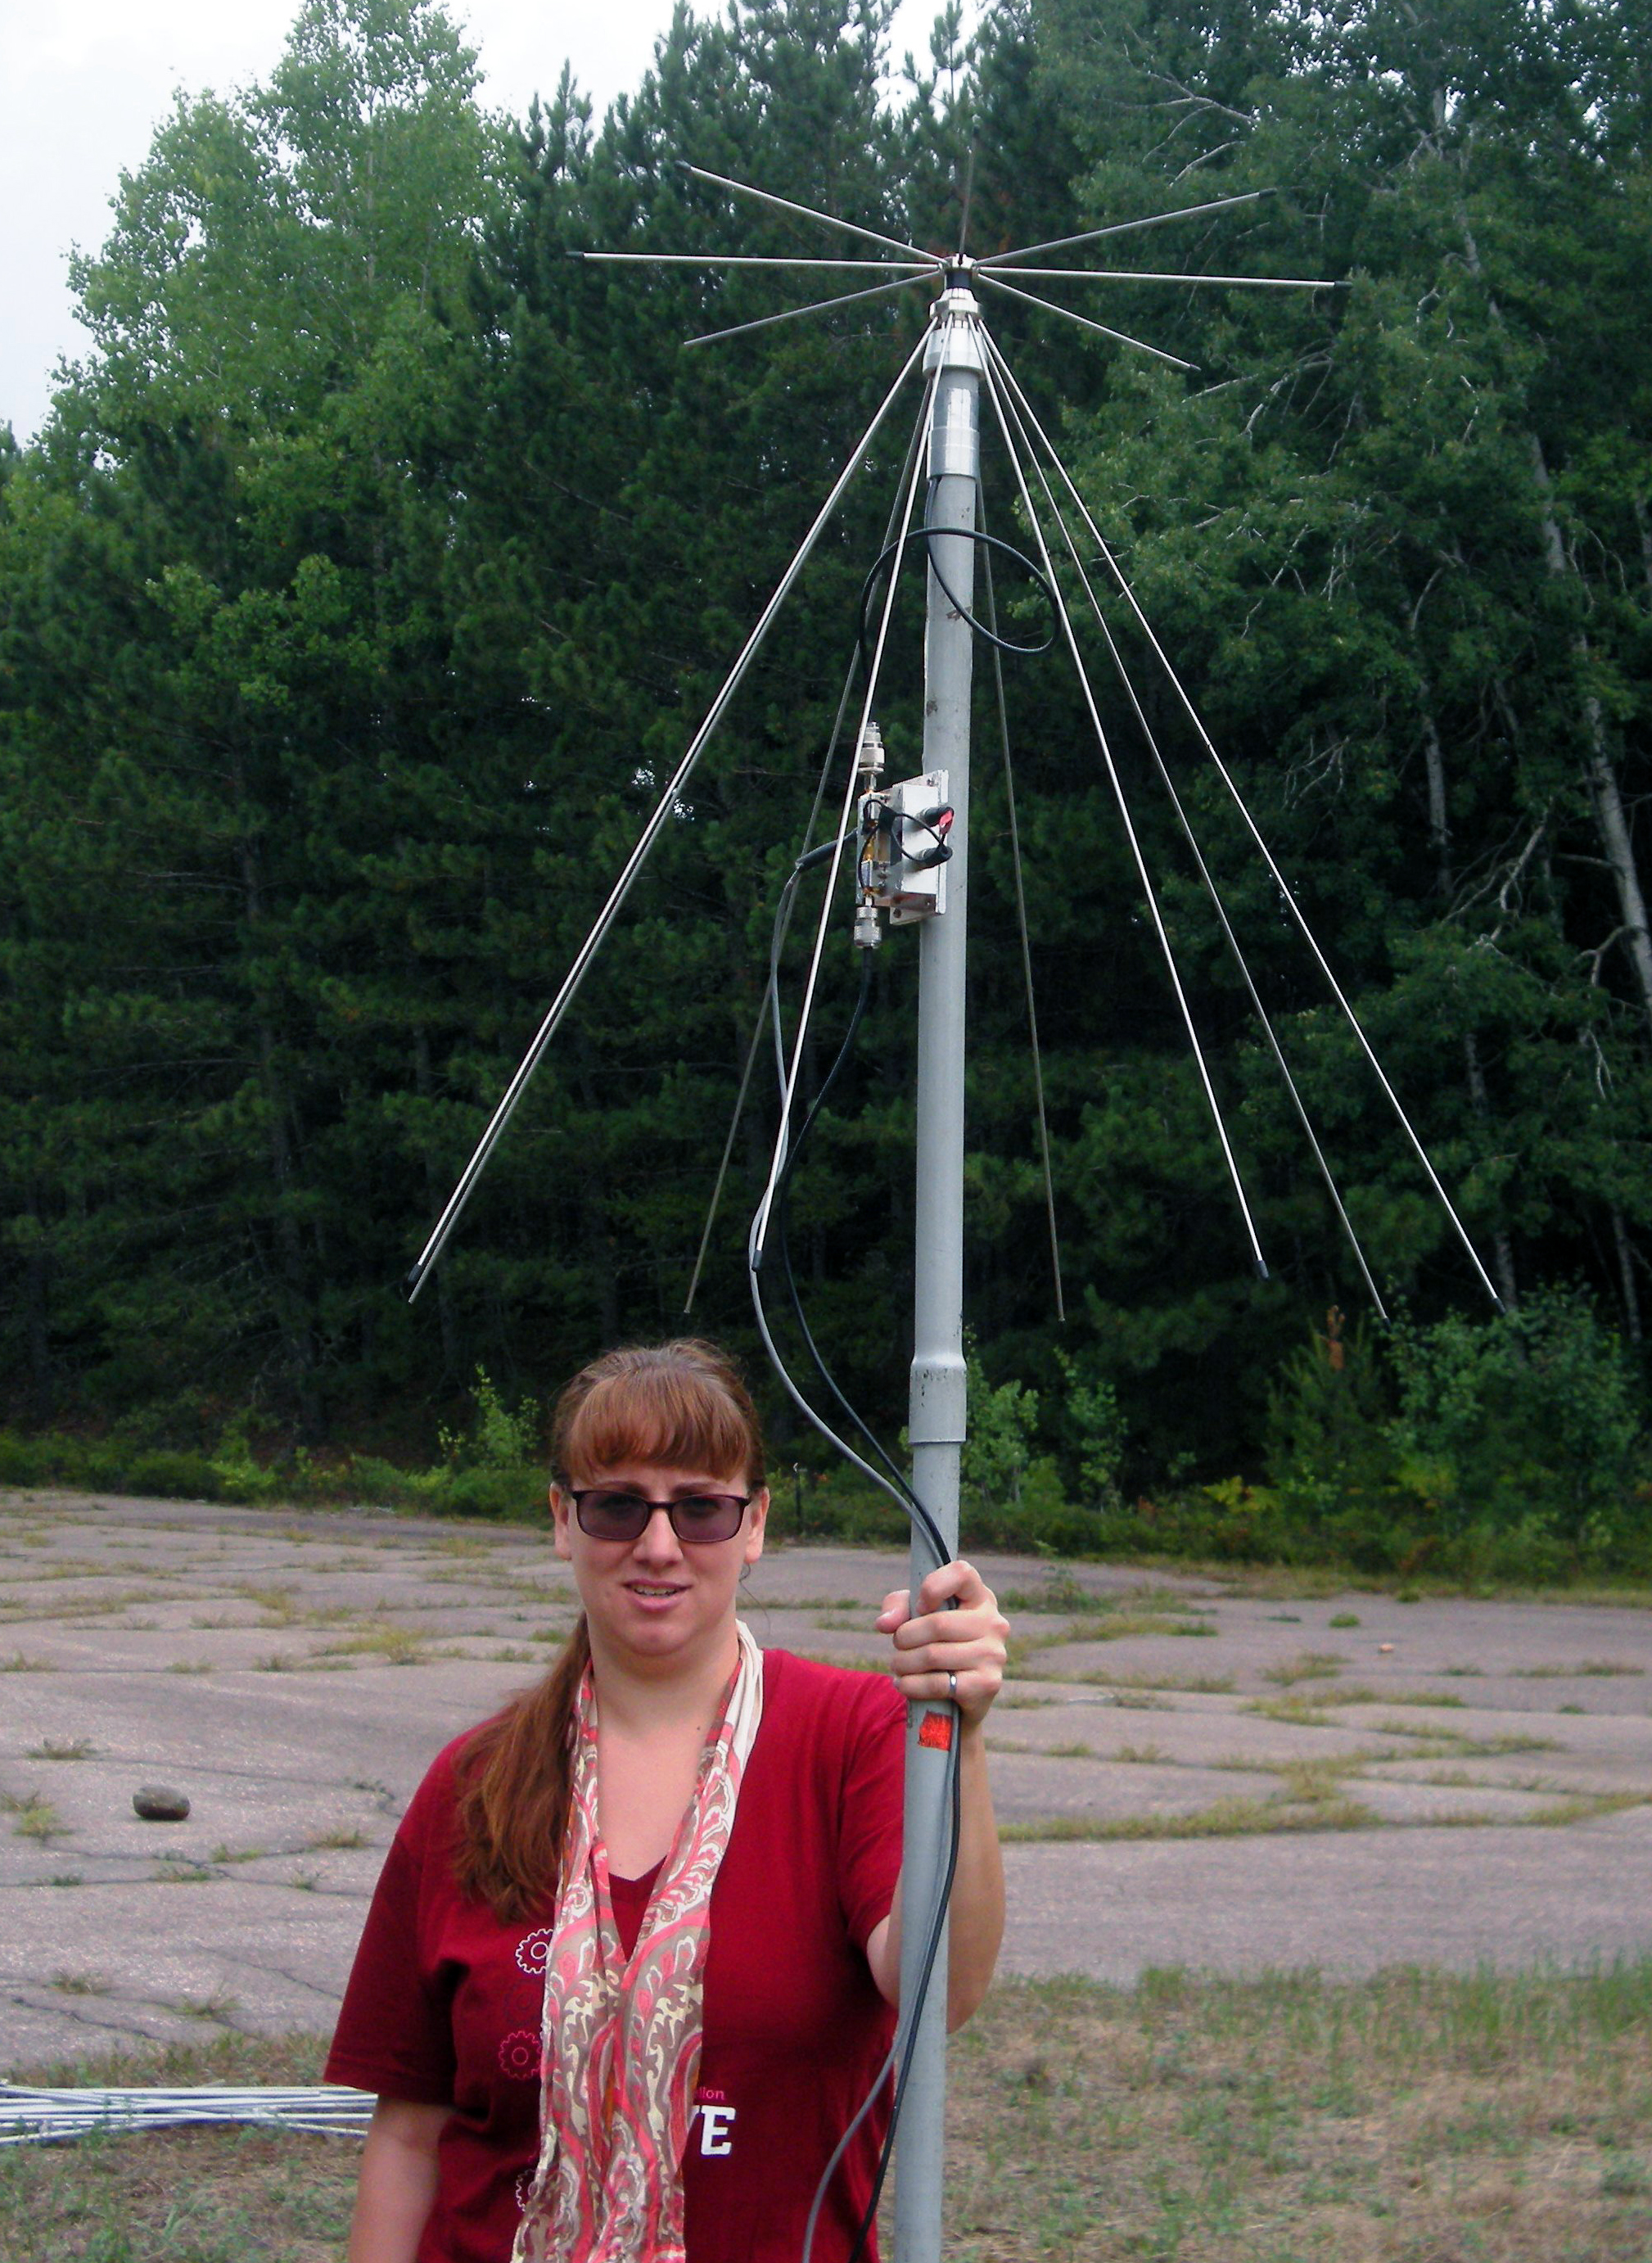
\includegraphics[width=0.95\linewidth]{RFI_testing/figures/voytek_site_test_alg.jpg}
\caption{Tabitha collecting RFI data with the site testing equipment while at one of the testing sites.}
\label{Fig:aroant}
\end{minipage}
\end{figure}

\begin{figure}[htb]
\begin{center}
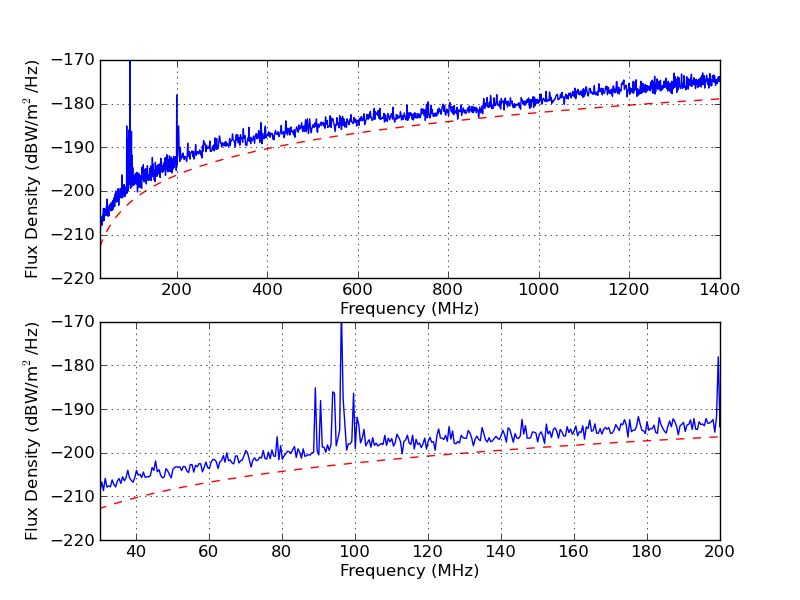
\includegraphics[width=0.9\linewidth]{RFI_testing/figures/50Ohm_cal.png}
\caption{Resistor measurement with the site testing kit. Blue line shows measured power from a $50 \Omega$ resistor. In the data, FM spikes are RF leakage due to the measurement being made in the lab in Pittsburgh where the FM band is extremely loud. Meanwhile, the red line is the expected signal level of a $50 \Omega$ resistor based on Equation \ref{eq:resflux}. The difference between the expected signal and actual signal can be attributed to limitations of the Spectrum Analyzer in measuring flux density.}
\label{Fig:resflux}
\end{center}
\end{figure}

\subsection{Site Testing Kit} \label{Sec:site_kit}

One major element of site evaluations was a set of single time sweep measurements of the RFI over a wide frequency band at each site. To do this, a site testing kit was assembled. The kit includes a broadband antenna, amplifiers, and a portable Spectrum Analyzer for data collection. 

RFI signals are received by the antenna and passed along the RF electronics into the Spectrum Analyzer. RFI is first received by the antenna, a Workman $T-601$ discone antenna with a vertical polarization and a 3 $m$ PVC pipe mast (see Figure \ref{Fig:aroant}). From the antenna, the received signal is then sent through a $50$ $cm$ cable to a set of amplifiers powered by a DC battery pack. The amplifiers are Minicircuits $ZX60-33LN$ followed by Minicircuits $ZX60-4016E$. The signal is then sent down a $\sim 7$ $m$ cable to the Spectrum Analyzer. The Spectrum Analyzer (Anritsu $MS2711A$) was enclosed in a brass mesh bag (Faraday Cage) to minimize self-generated RF contamination. 

Data is collected by sweeping individual $200 MHz$ bands from $\sim1 MHz$ to $1600 MHz$, with a video and resolution bandwidth of $100 kHz$. Only 400 data points are saved by the Spectrum Analyzer, requiring the data to be rebinned down to $500 kHz$ resolution. The highest peak of the $\sim50$ data points within each $500 kHz$ band is stored, which can be accounted for by changing the resolution bandwidth to an effective bandwidth of $30 kHz$. 

In order to convert the data to flux density (S in $dB \; W/m^2Hz$), Equation \ref{eq:fluxdens} was applied to the data. In the equation, $G$ is the amplifier gain in dB, $BW$ is the effective spectrum analyzer bandwidth in $Hz$ and $G_{ant}$ is the antenna gain in dB. 

\begin{equation}\label{eq:fluxdens}
S \Bigg( \frac{dB \; W}{m^2 Hz} \Bigg) = P_{meas} (dBm) - 30 \Bigg( \frac{dB \; W}{dB \;m} \Bigg) - G - 10log_{10} [BW] - G_{ant}
\end{equation}

Amplifier gain ($G$) was measured in the lab using a noise figure meter and antenna gain ($G_{ant}$) can be calculated using Equation \ref{eq:gant}, where $\nu$ is the frequency in $Hz$, and $A_g$ is the isotropic antenna gain in $m^2$. We used a value for $A_g$ corresponding to the typical value for our antenna, which is $1 dB \;i$ or $10^{1dB \;i/10} m^2$. 

\begin{equation}\label{eq:gant}
G_{ant}= 10 log_{10} \Bigg[ \Bigg(\frac{c}{\nu} \Bigg)^2 \Bigg( \frac{A_g}{4 \pi} \Bigg) \Bigg]
\end{equation}

To test the conversion equation, we replaced the antenna with a $50 \Omega$ resistor. That resistor should have a flux density which can be calculated using Equation \ref{eq:resflux}, where $k$ is the Boltzmann Constant, $T$ is the room temperature in Kelvin and $NF$ is the amplifier noise as measured using a noise figure meter. 

\begin{equation}\label{eq:resflux}
S \Bigg( \frac{dB \; W}{m^2 Hz} \Bigg) = 10 log_{10} [k T] + NF 
\end{equation}

\begin{figure}[tb]
\begin{center}
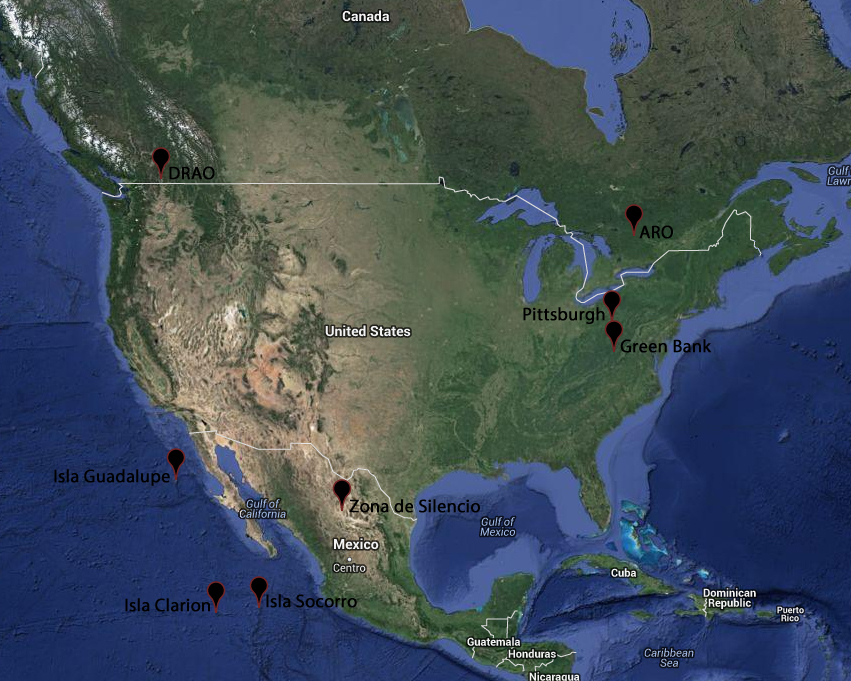
\includegraphics[width=0.95\textwidth]{RFI_testing/figures/large_scale_site_map.jpg}
\caption{Map of evaluated sites in North America, created using Google Maps.}
\label{Fig:site_map}
\end{center}
\end{figure}

The results of this measurement are shown in Figure \ref{Fig:resflux}. The measured signal was slightly higher than expected signal. Some of this difference was tied to the effective Spectrum Analyzer bandwidth ($30 kHz$), which is larger than the $10 kHz$ bandwidth quoted in the analyzer specifications from the manufacturer. The remainder of the difference may come from additional noise in the system or uncertainty in the noise figure meter values, but it is roughly flat in frequency. 

Because we use the same kit at all the sites, any systematic noise contribution such as the uncertainty in the $50 \Omega$ data found in Figure \ref{Fig:resflux} is constant across all datasets. 

\begin{figure}[tb]
\begin{center}
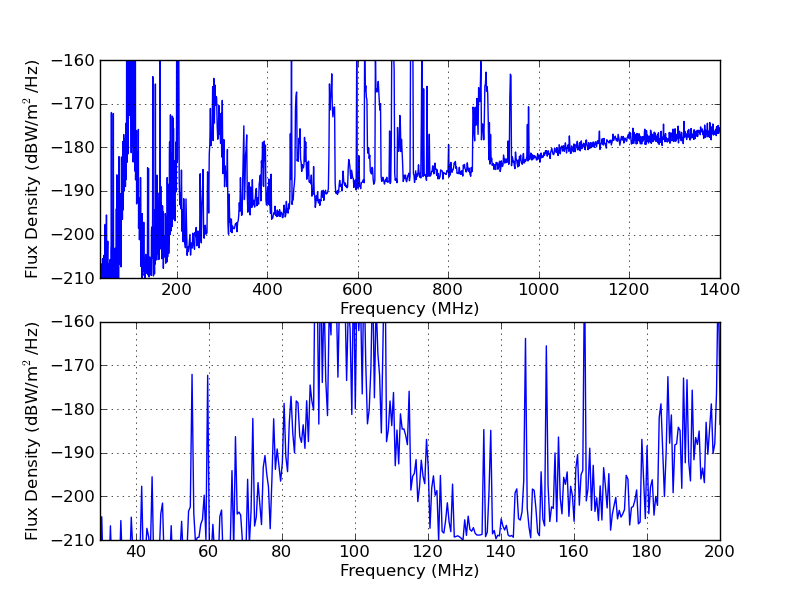
\includegraphics[width=0.9\linewidth]{RFI_testing/figures/Pittsburgh_cal.png}
\caption{RFI measurement at Carnegie Mellon University in Pittsburgh, Pennsylvania collected April 23rd, 2009. In the data, there are many RFI sources that produce signals that have a magnitude above the plotted range. These strong RFI signals produce inter-modulations that corrupt data outside of the actual frequencies of the RFI. For example, strong FM signals cause inter-modulation below  $88 MHz$ and above $108 MHz$. }
\label{Fig:pghcal}
\end{center}
\end{figure}



\section{Existing Site Evaluations}

Using the site testing kit discussed in Section \ref{Sec:site_kit}, data was taken at each of the sites shown in Figure \ref{Fig:site_map}. The portability of the kit (it packs up into the small suitcase and poster tube shown in Figure \ref{Fig:site_kit}) allows it to be easily transported to each of the sites. 


\subsection{Carnegie Mellon University Pittsburgh, PA, USA}

Carnegie Mellon University is located in the city of Pittsburgh ($40^\circ 26'30''$ N, $80^\circ 00' 00''$ W), home to several universities and possessing a population of over 300,000. As should be expected, the radio environment in Pittsburgh is full of RFI with signals of such magnitude that they overload test equipment. Figure \ref{Fig:pghcal} shows the RFI environment in Pittsburgh as measured with the site testing kit. The RFI signals are so loud in Pittsburgh that they overload the Spectrum Analyzer. 

To try and lower the RFI levels to measurable levels, we removed one stage of amplification from the system for the low frequency data. This is why the noise floor in Figure \ref{Fig:pghcal} is lower at low frequencies than it is in the other datasets. Amplification removal was designed to minimize the inter-modulation which begins to occur when there are RFI signals larger than $-170 \frac{dB \;W}{m^2 Hz}$. However, even with the amplifier removed from the system some of the RFI signals were still above the inter-modulation cutoff. For example, strong FM signals cause inter-modulation below $88 MHz$ and above $108 MHz$ in the Pittsburgh data. 


\begin{figure}[htb]
\centering
\begin{minipage}[b]{0.47\textwidth}
\centering
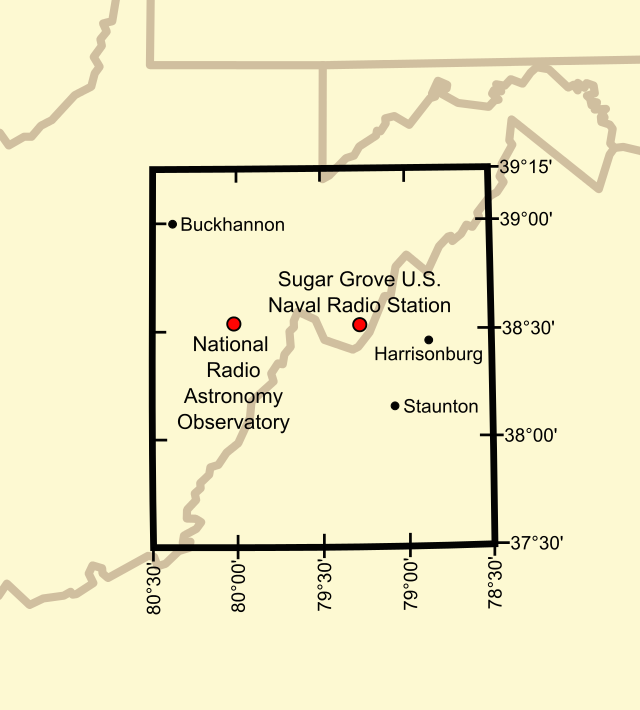
\includegraphics[width=0.75\linewidth]{RFI_testing/figures/National_Radio_Quiet_Zone.png}
\caption{Extent of the U.S. National Radio Quiet Zone around the Green Bank Site.}
\label{Fig:nrqz}
\end{minipage}%
\begin{minipage}[b]{0.02\textwidth}
\hspace{1cm}
\end{minipage}%
\begin{minipage}[b]{0.47\textwidth}
\centering
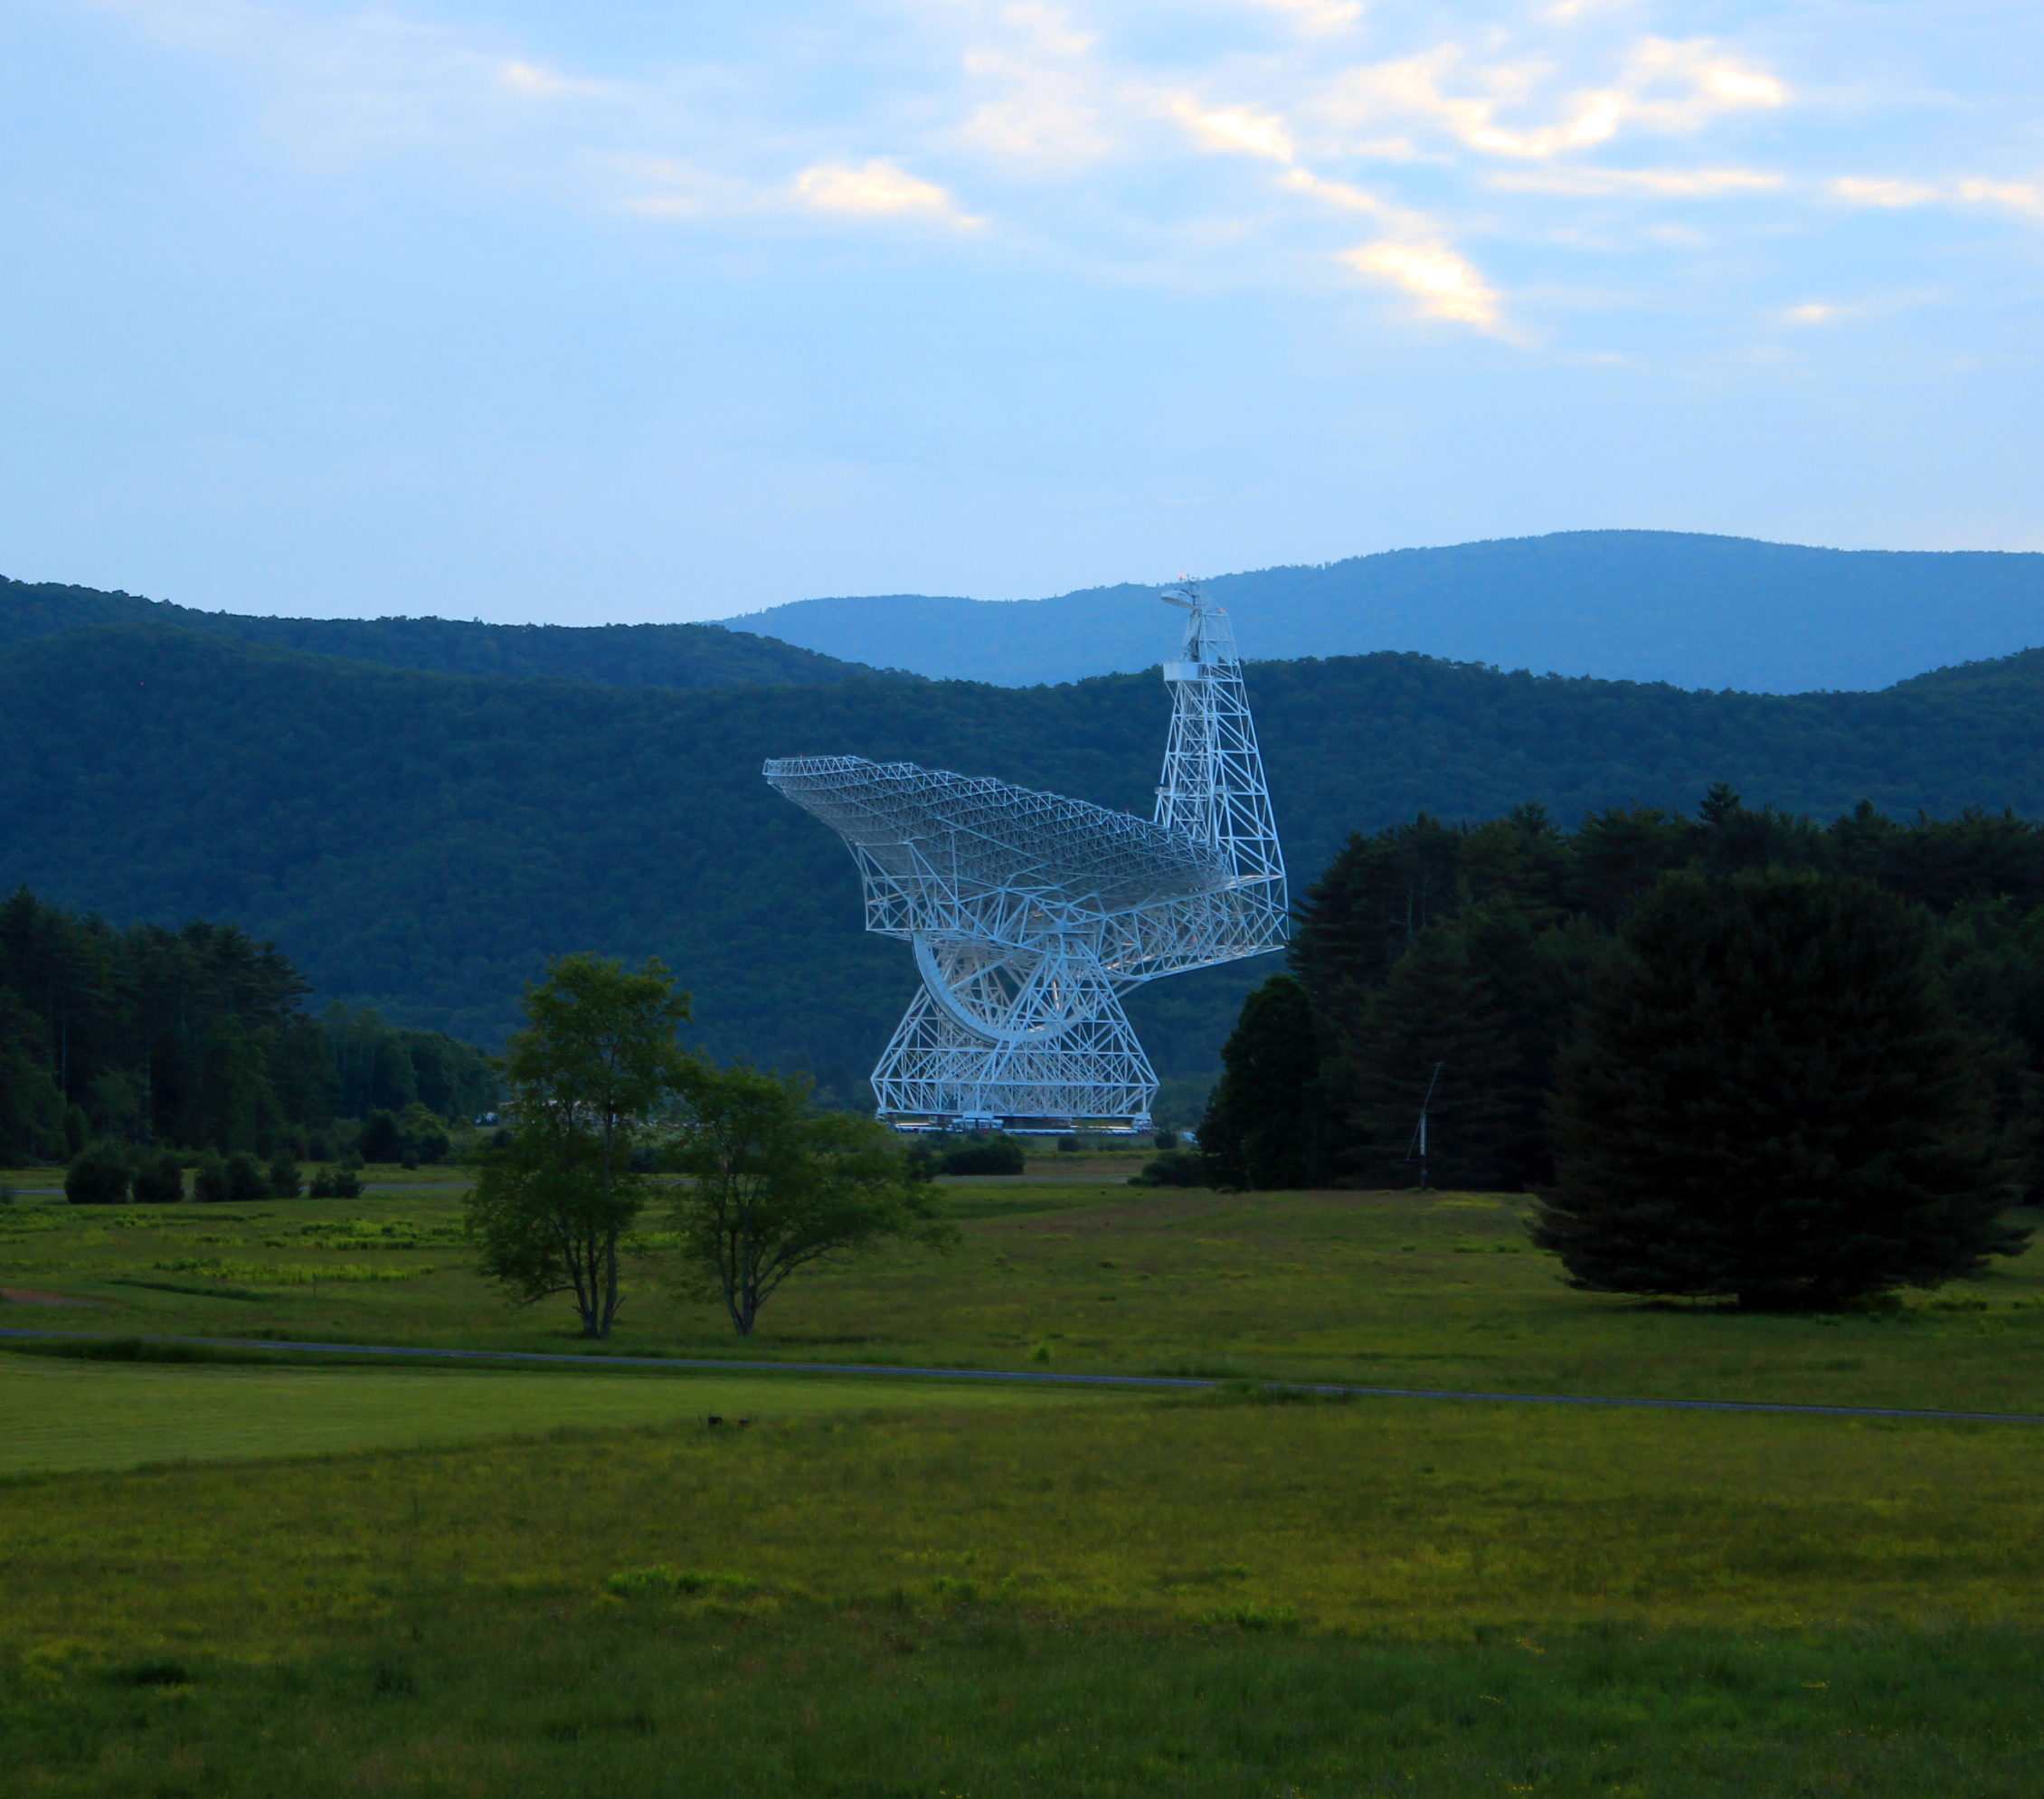
\includegraphics[width=0.95\linewidth]{RFI_testing/figures/gbt_site.jpg}
\caption{Robert C. Byrd Green Bank Radio Telescope as viewed from the site observation deck. }
\label{Fig:gbt}
\end{minipage}
\end{figure}

\begin{figure}[htb]
\begin{center}
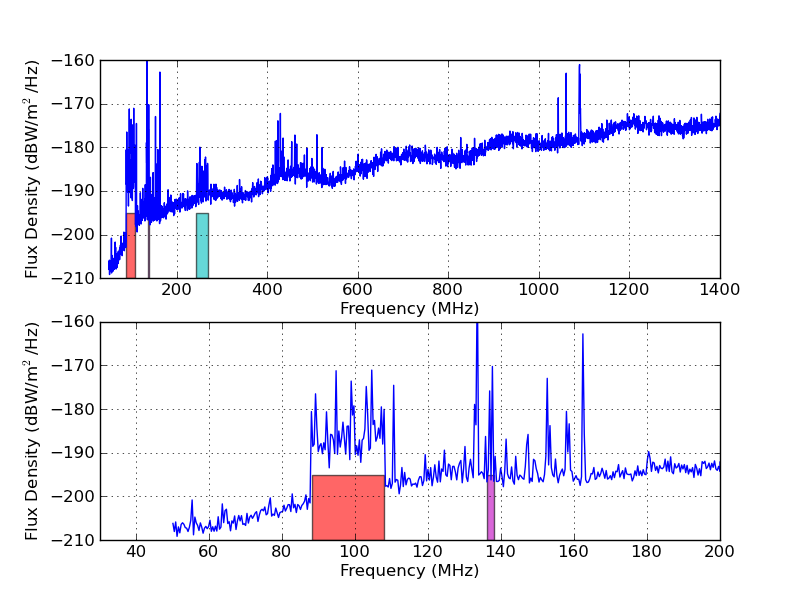
\includegraphics[width=0.9\linewidth]{RFI_testing/figures/GBT_bands.png}
\caption{RFI measurement at the NRAO Green Bank site collected on May 18th, 2010. In the plot, colored boxes indicate bands of well known RFI sources. Red is the FM band, Purple is the Orbcomm satellite band, and Cyan is the military satellite band. Additional spikes in the data come from RFI sources not in the indicated bands. Large scale sinusoidal variation (or ringing) in the spectrum is caused by cable reflections in the system and is common to all data collected with the site testing kit. }
\label{Fig:gbtrfi}
\end{center}
\end{figure}


\subsection{National Radio Astronomy Observatory (NRAO) Green Bank}

The National Radio Astronomy Observatory (NRAO) is a research center funded by the U.S. National Science Foundation (NSF). It maintains several telescopes in radio quiet locations. One of these locations is in Green Bank, West Virginia inside the U.S. National Radio Quiet Zone in Virginia and West Virginia (see Figure \ref{Fig:nrqz}). Within this zone, radio broadcasts at all frequencies are minimized by law. This provides a relatively quiet RFI environment. 

The Green Bank site ($38^\circ 25' 59''$ N, $79^\circ 50' 23''$ W) hosts a number of radio telescopes including the $100 \; m$ Robert C. Byrd Green Bank Radio Telescope (see Figure \ref{Fig:gbt}). As an NRAO facility, the site has a full staff and facilities including housing, power, and other amenities. Located off a local highway, the site is a 4-5 hour drive from Pittsburgh. 

Looking at the data from the site testing kit, we find that the size of the radio quiet zone (about 34,000 $km^2$) is sufficient for higher frequencies but is too small at lower frequencies. As you can see in Figure \ref{Fig:gbtrfi}, there are specific bands of frequencies below $600 MHz$ where there is still a great deal of RFI. Some of these bands are indicated with colored boxes (red is the FM band, magenta is an Orbcomm satellite band and cyan is a military satellite band). 

Beyond the RFI, one of the other features of the site test data is a large scale sinusoidal variation (or ringing) in frequency. This variation is caused by reflections in the $50 \; cm$ cable between the antenna and first stage amplifier. One of the useful things about this ringing is that it provides a check that the system is working, because if one or more of the amplifiers has blown there is no ringing present in the data. Such a cross check is particularly useful in radio quiet areas, where there may not be much of a difference in the spectrum if the amplifier is malfunctioning. 

\begin{figure}[htb]
\begin{center}
\includegraphics[width=0.9\linewidth]{RFI_testing/figures/penticton_rect.jpg}
\caption{Some of the DRAO facilities and telescopes (CHIME pathfinder in foreground). }
\label{Fig:penticton}
\end{center}
\end{figure}

\begin{figure}[htb]
\begin{center}
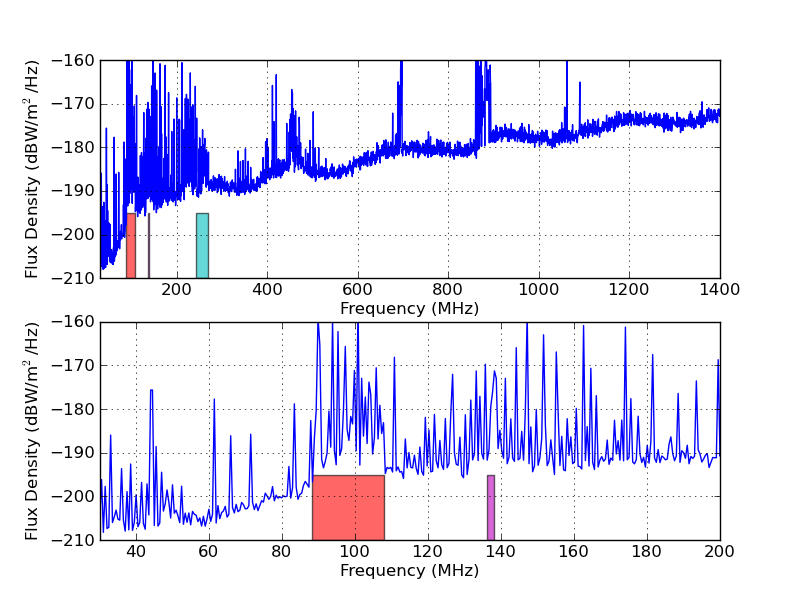
\includegraphics[width=0.9\linewidth]{RFI_testing/figures/DRAO_bands.png}
\caption{RFI measurement at the DRAO Penticton site collected on December 14th, 2009. DRAO has excessive RFI in the entire spectrum below $400 MHz$ and is generally noisier than Green Bank. Because some of these signals (particularly the FM band) are above the inter-modulation cutoff, some of the smaller spikes in known clear bands are believed to be caused by inter-modulation. In the plot, colored boxes again indicate bands of well known RFI sources (Red= FM band, Purple = Orbcomm satellite band, and Cyan = military satellite band).   }
\label{Fig:draorfi}
\end{center}
\end{figure}

\begin{figure}[tb]
\begin{center}
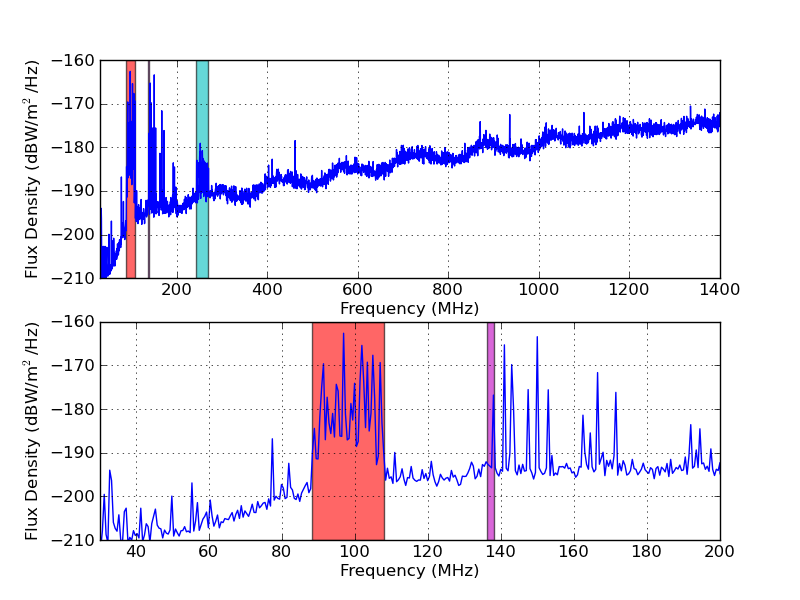
\includegraphics[width=0.9\linewidth]{RFI_testing/figures/ALG_bands.png}
\caption{RFI measurement at the ARO Algonquin site collected on September 12th, 2012. Like the GBT site, the ARO site is quiet at high frequencies compared to DRAO or Pittsburgh. However, significant RFI is still present below $300 MHz$. In the plot, colored boxes again indicate bands of well known RFI sources (Red= FM band, Purple = Orbcomm satellite band, and Cyan = military satellite band).}
\label{Fig:arorfi}
%\end{minipage}
\end{center}
\end{figure}


\subsection{Dominion Radio Astrophysical Observatory (DRAO)}

The Dominion Radio Astrophysical Observatory (DRAO) is a Canadian radio astronomy site ($49^\circ 19' 15.6''$ N, $119^\circ 37' 26.4''$ W). Located near Penticton, British Columbia in the south-central part of the province, DRAO has a number of radio telescopes on site and the Canadian Hydrogen Intensity Mapping Experiment (CHIME) system is currently being built there. Figure \ref{Fig:penticton} shows some of the facilities at DRAO including part of the CHIME pathfinder in the foreground. 

The site can be easily accessed by car, with on-site facilities available for researchers. It is also a $\sim$30 minute drive from Penticton, a town with a population of over 30,000. 

Like the NRAO Green Bank site, the DRAO site has insufficient isolation from civilization to provide a radio quiet environment at the lower frequencies. There is significant RFI contamination for most frequencies below $500 MHz$ at this site (see Figure \ref{Fig:draorfi}). Given DRAO's location close to Penticton, some of the signals in the FM band are loud enough to cause intermodulation of signals into some of the frequencies that are actually clean. This can be seen in the band between $108-136 MHz$, the dedicated aerospace band, which should be clear of RFI everywhere in the world. 


\subsection{Algonquin Radio Observatory (ARO)}

The Algonquin Radio Observatory (ARO) is a single instrument Canadian radio astronomy site ($45^\circ 57' 19.8''$ N, $78^\circ 4' 23''$ W). Located in the center of Algonquin Provincial Park in Ontario, Canada; the site is only accessible by logging roads, which are gravel but can be driven by most vehicles during the summer. ARO is also accessible in an emergency via helicopter, but this mode of transportation is not commonly used. ARO does have power and full amenities on site including housing for researchers. 

Although the site has excellent radio quiet properties at higher frequencies, it is still relatively close (about $200-250 \; km$) to the major Canadian metropolitan areas of Toronto and Ottawa. When we set up our site test at ARO, we found that although the rest of the spectrum is quite clean there is still significant RFI below $300 MHz$ (see Figure \ref{Fig:arorfi}), including in the FM radio band. 


\begin{figure}[htb]
\begin{center}
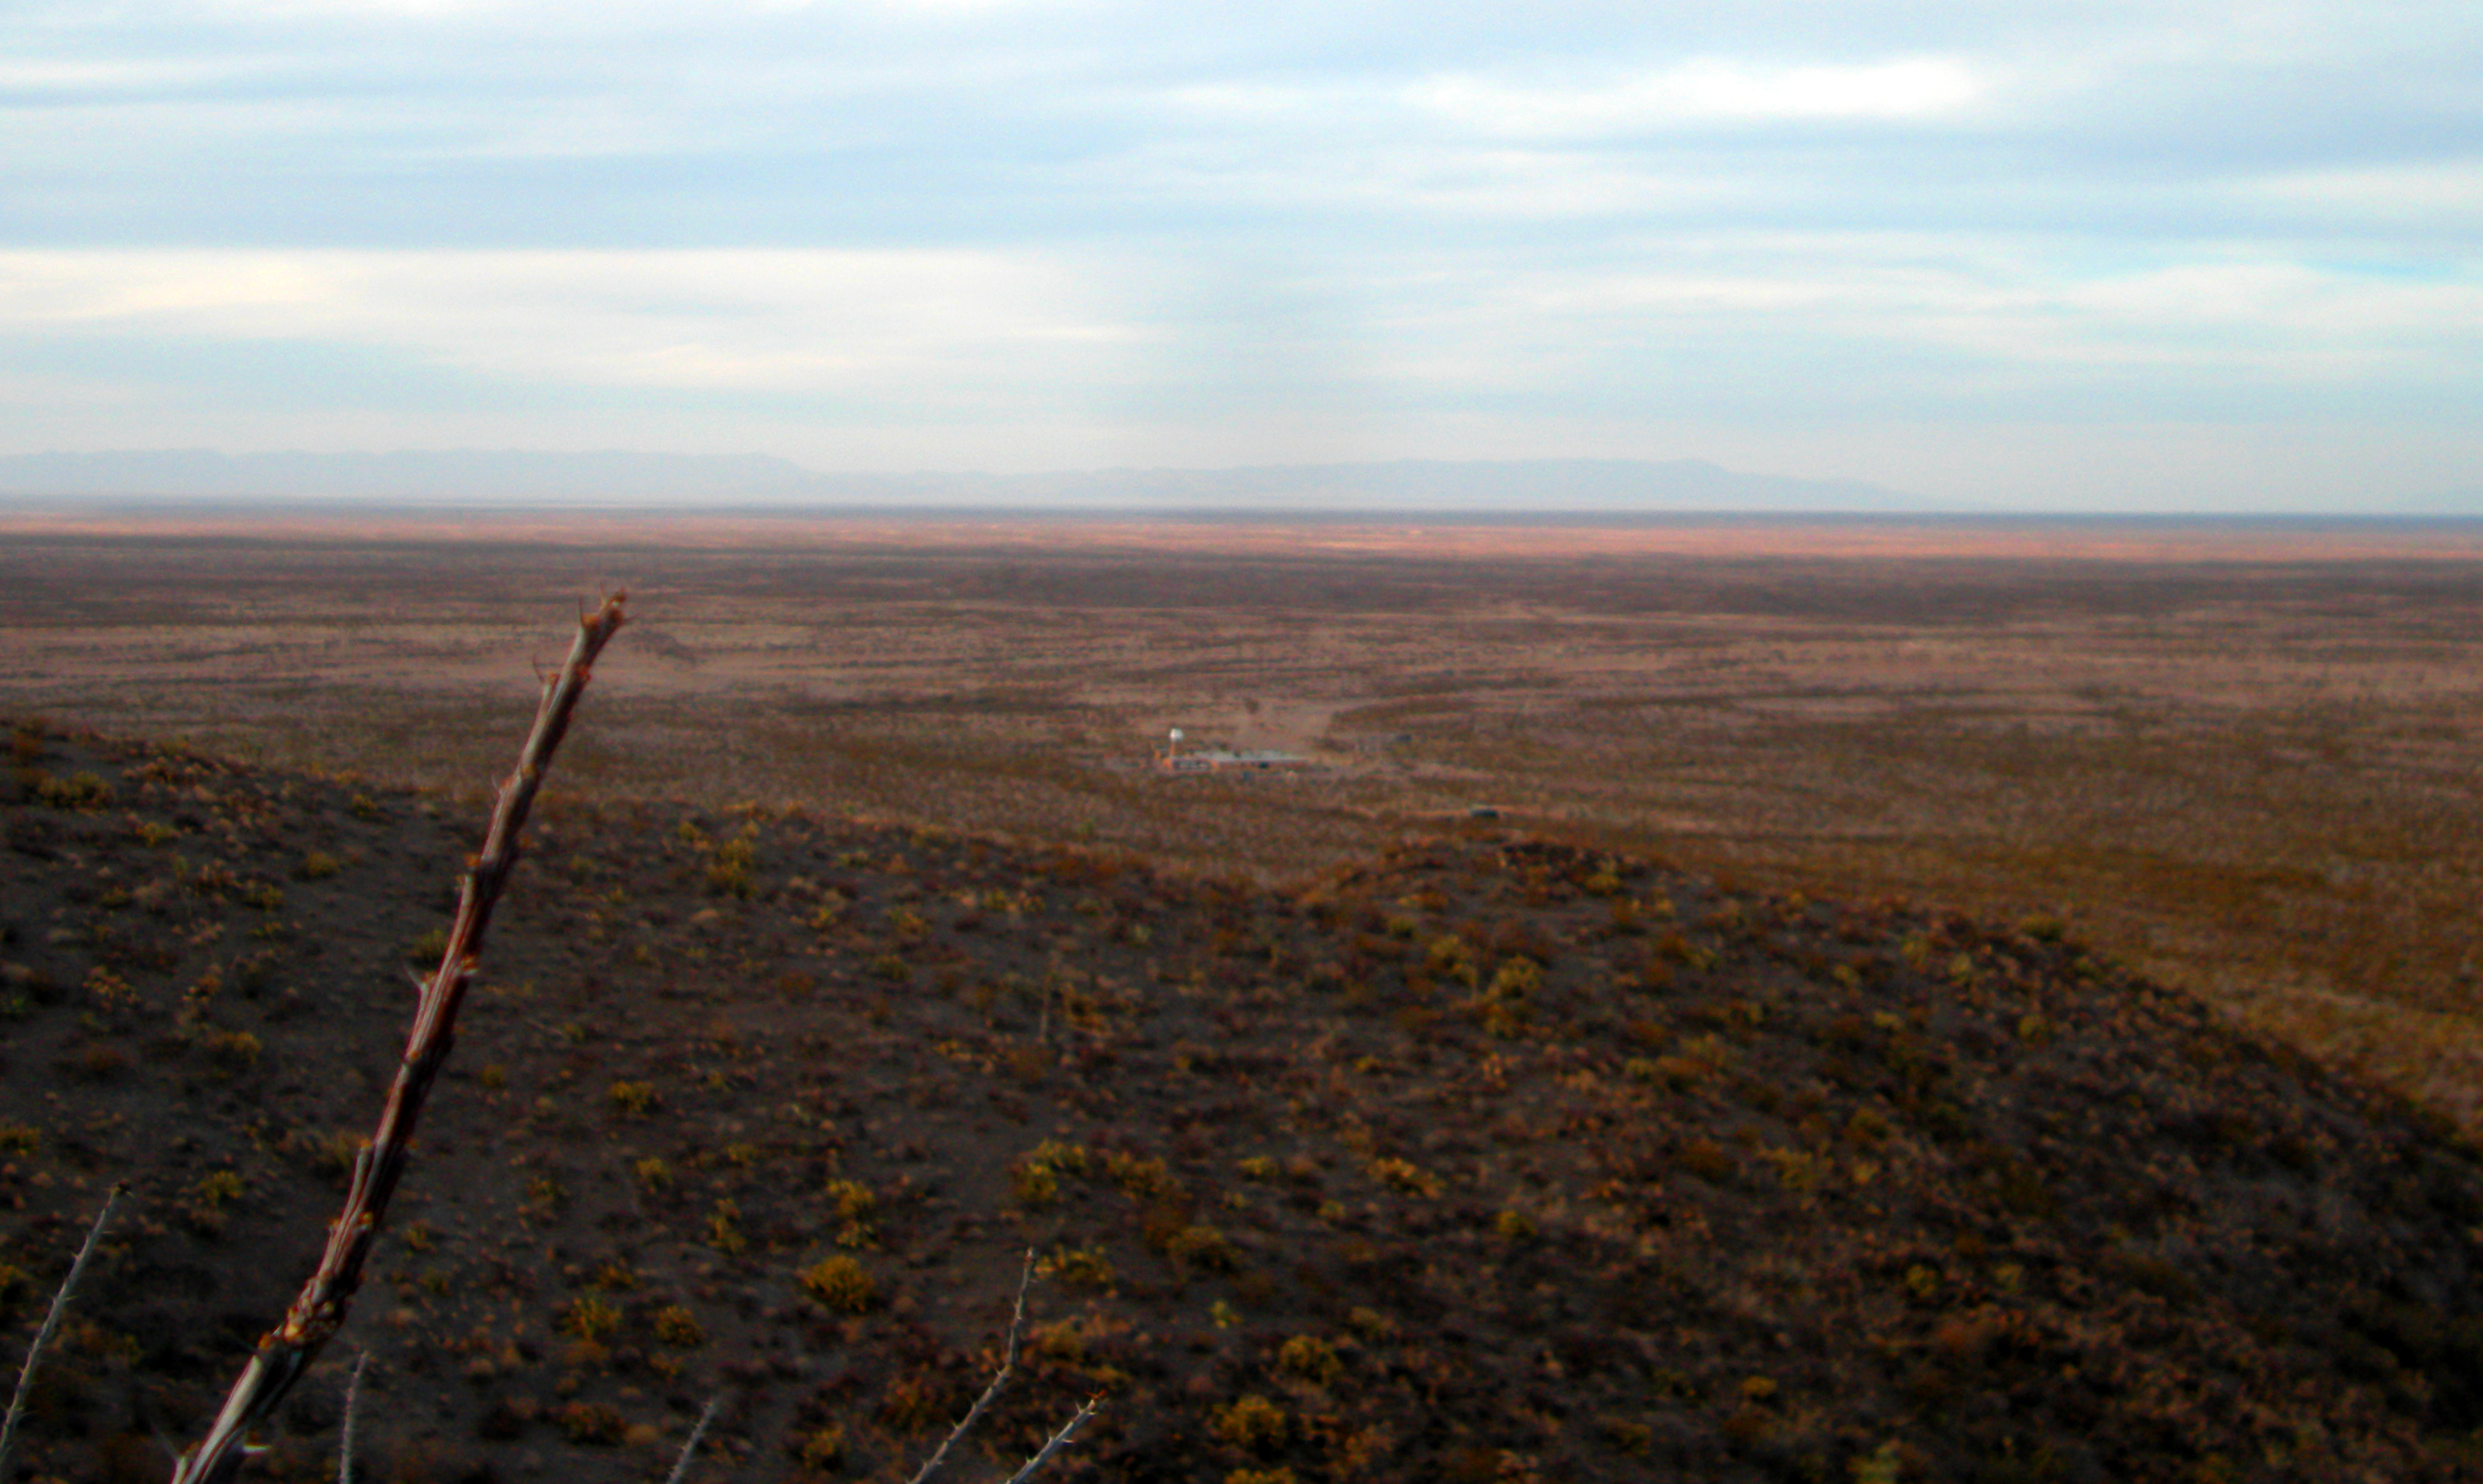
\includegraphics[width=0.9\linewidth]{RFI_testing/figures/zds_overview_shot.jpg}
\caption{View of the Zona del Silencio from one of the nearby peaks. The ecologist's camp where we stayed while running our tests is in the center of the picture.}
\label{Fig:zdsover}
\end{center}
\end{figure}

\begin{figure}[htb]
\begin{center}
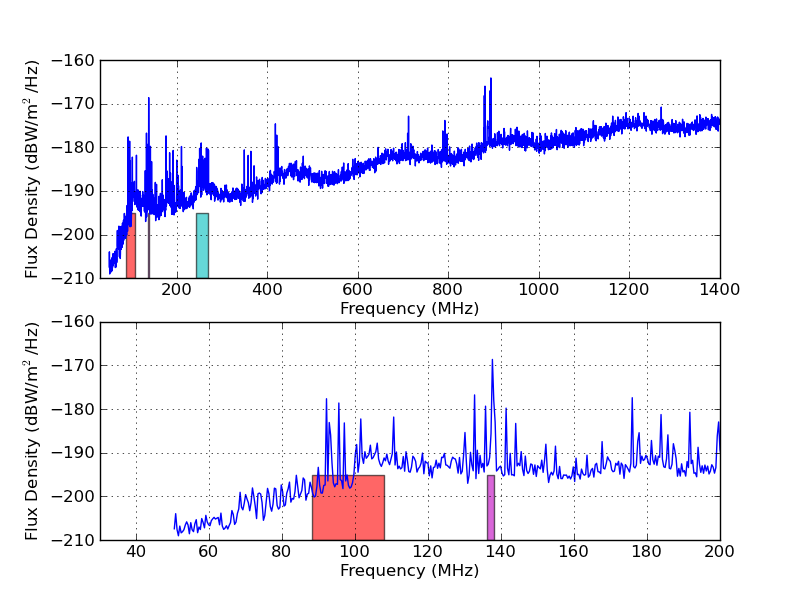
\includegraphics[width=0.9\linewidth]{RFI_testing/figures/ZdS_halfway_in_bands.png}
\caption{RFI measurement near the ecologist's camp in the Zona del Silencio, collected on May 5th, 2010. The Zona del Silencio site has even less RFI than the previous sites at low frequencies, although some RFI spikes are still present. In the plot, colored boxes again indicate bands of well known RFI sources (Red= FM band, Purple = Orbcomm satellite band, and Cyan = military satellite band).}
\label{Fig:zdsendrfi}
\end{center}
\end{figure}



\section{New Site Evaluations}

Evaluation of these existing radio quiet sites demonstrated a clear need for sites whose RFI environments are cleaner at frequencies below $500 MHz$. However, locating such sites can be difficult as the distances required begin to grow large. Here, I report on a couple of potential sites in Mexico that have significant improvement in their low frequency RFI strength compared to the existing sites. 


\subsection{La Zona del Silencio}

$''$Zona del Silencio$''$ ($26^\circ 41' 10.3''$ N, $103^\circ 44' 50.9''$ W) is a radio quiet region in the Mapimi part of the Chihuahuan desert in Northern Mexico. It has a reputation as a mysterious radio quiet zone due to historic events similar to the Bermuda Triangle, but in a desert setting. Some of its radio quiet status may be due to the local geography as the desert is a flat plateau, but there are mountains between it and any significant civilization. The closest major metropolitan area is Torre\'{o}n, over $150 km$ south of the zone center. The zone is also a protected biosphere reserve maintained by Mexico's $''$Comisi\'{o}n Nacional de \'{A}reas Naturales Protegidas$''$ (CONANP). 

\subsubsection{Logistics and Current Infrastructure}

While major highways can be found along the outside of the region, the only roads in and out of the site are poorly maintained dirt roads that require 4-wheel drive.

Permanent settlements are not allowed within the biosphere reserve. However, at the center of the site is a camp for ecologists studying the biosphere found in the reserve. The site has minimal housing with solar cells charging batteries for power but all water on site has to be brought in from outside. 

For our site test, we got special permission to stay at the ecologist's camp called $''$Laboratorio del Desierto$''$, shown in Figure \ref{Fig:zdsover}.

\subsubsection{Environmental Impacts}

During the site testing, we were able to observe the general climate of the site as a consideration for future deployments. One of the challenges we observed was the prevalence of dust due to the arid climate. All our equipment had to be well protected from dust, especially during transport to and from the site. If not properly shielded, dust can cause electronic equipment to malfunction. 

Another potential challenge is the temperature variation associated with the climate. Even within a single day we saw a strong difference between night and day temperatures. Temperature variation can create variance in collected data from a telescope, making the desired signals more difficult to detect. 

\subsubsection{Measurements}

On this first site test, we chose to measure the site quality at a specific location near the center of the zone where RFI was expected to be at a minimum. Setting up near the ecology camp but far enough away to prevent contamination by the local electronics, we measured extremely low RFI levels as is shown in Figure \ref{Fig:zdsendrfi}.

There is still some noise at lower frequencies, but the FM band is considerably quieter than at any of the existing radio quiet sites that we had tested. Further testing at this site should include a survey of a wide range of locations within the $''$Zona del Silencio$''$ to map out the region's radio quiet properties. 

\begin{figure}[htb]
\centering
\begin{minipage}[b]{0.47\textwidth}
\centering
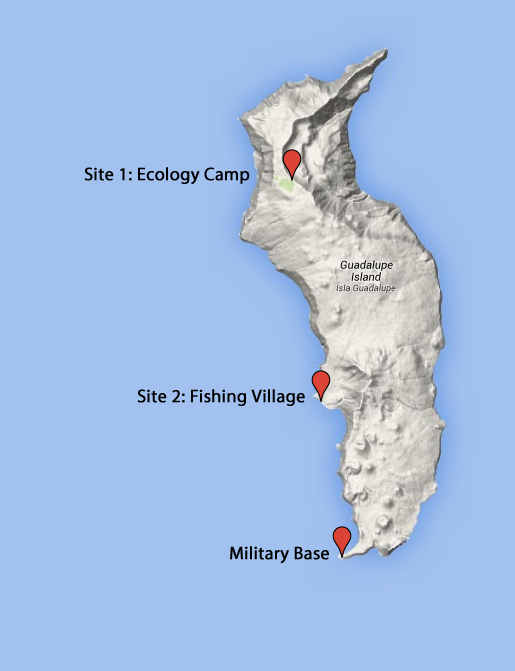
\includegraphics[width=0.93\linewidth]{RFI_testing/figures/isla_guadalupe_site_map.jpg}
\caption{Map of Isla Guadalupe showing the sites of interest, made using Google Maps. }
\label{Fig:guadmap}
\end{minipage}%
\begin{minipage}[b]{0.02\textwidth}
\hspace{1cm}
\end{minipage}%
\begin{minipage}[b]{0.47\textwidth}
\centering
\includegraphics[width=0.95\linewidth]{RFI_testing/figures/omar_site_test_guad.jpg}
\caption{Collecting data with the site testing equipment on Isla Guadalupe.}
\label{Fig:guadsite}
\end{minipage}
\end{figure}


\begin{figure}[htb]
\centering
\begin{minipage}[b]{0.455\textwidth}
\centering
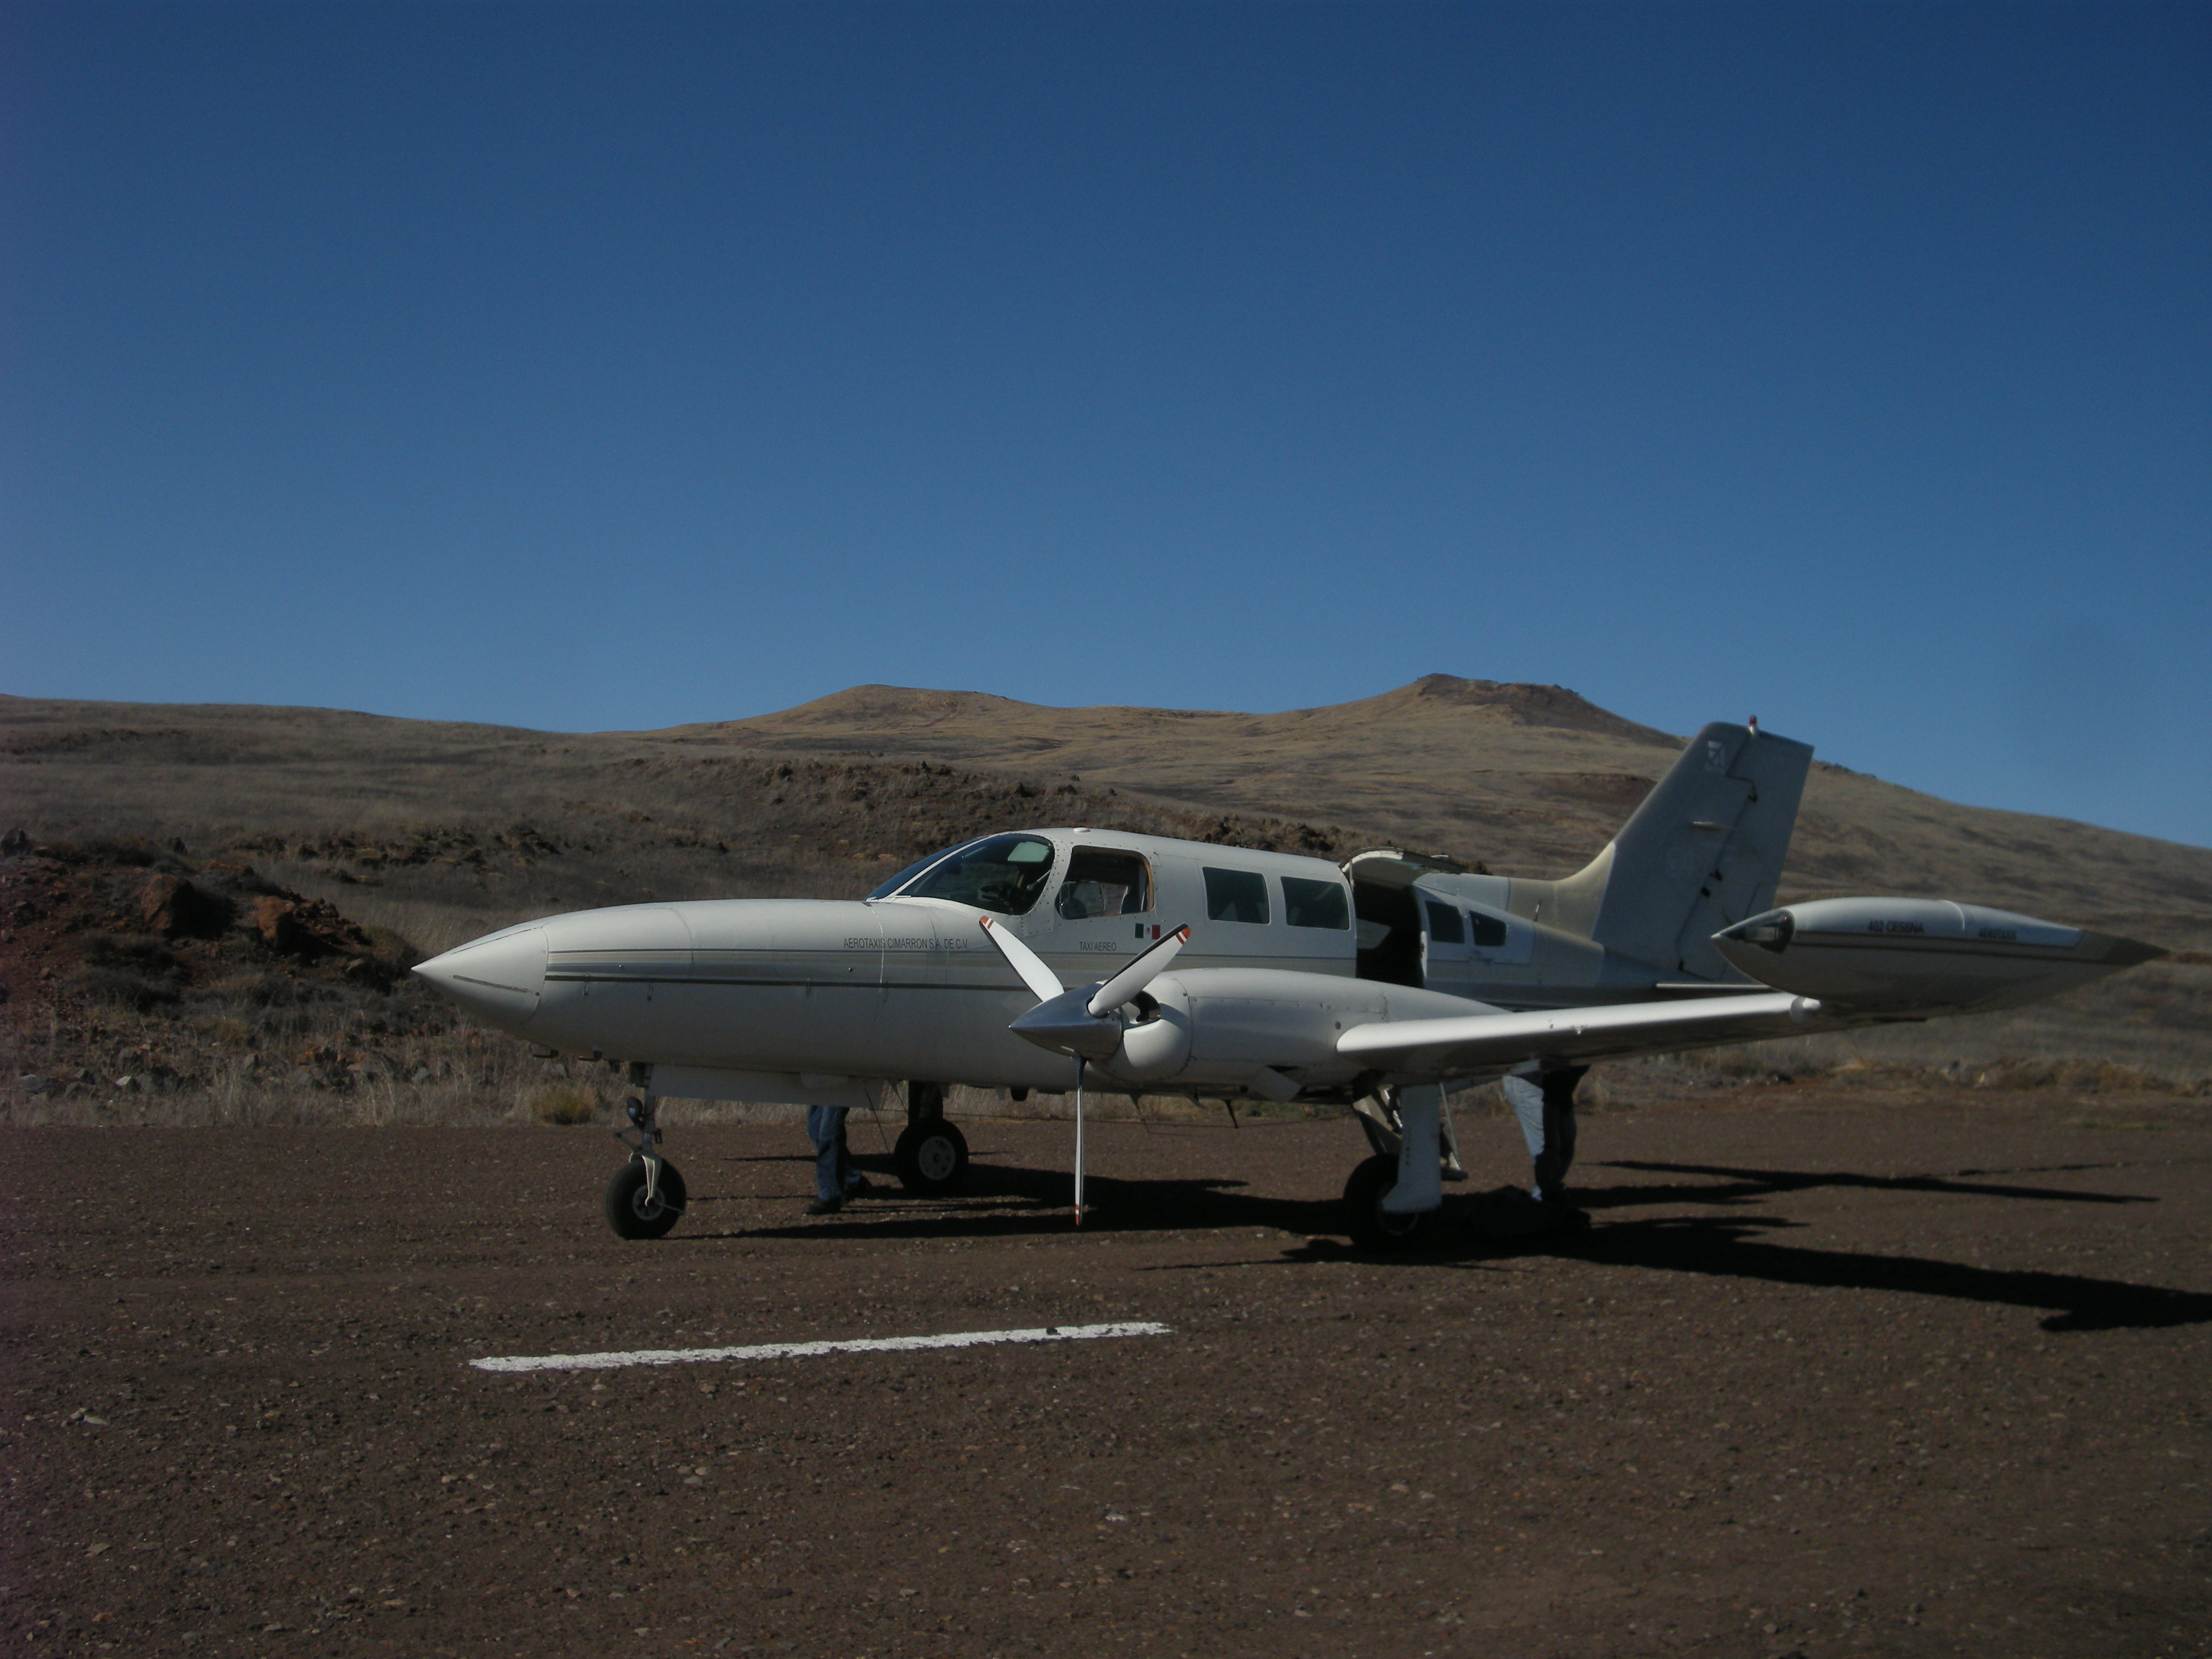
\includegraphics[width=0.95\linewidth]{RFI_testing/figures/guad_plane.jpg}
\caption{Airplane used for access to Isla Guadalupe.}
\label{Fig:guadplane}
\end{minipage}%
\begin{minipage}[b]{0.02\textwidth}
\hspace{1cm}
\end{minipage}%
\begin{minipage}[b]{0.485\textwidth}
\centering
\includegraphics[width=0.95\linewidth]{RFI_testing/figures/guad_plateau_plane.jpg}
\caption{View of the plateau with the fishing village from the airplane.}
\label{Fig:guadplateau}
\end{minipage}
\end{figure}


\subsection{Isla Guadalupe}

Isla Guadalupe ($29^\circ 1' 51''$ N, $118^\circ 16' 48''$ W) is a small volcanic island located about 250 $km$ west of Baja California in Mexico. The island has an area of $\sim$250 $km^2$, with two significant peaks along the north-south axis of the island. A biosphere reserve, access to Guadalupe is limited to a few groups. Namely, the Mexican government and Navy ($''$Secretar\'{i}a de Gobernaci\'{o}n$''$ and $''$Secretar\'{i}a de Marina$''$), ecologists studying the land and marine life such as the $''$Grupo de Ecolog\'{i}a y Conservaci\'{o}n de Islas A.C.$''$ (GECI) and CONANP, and the local fishing cooperative ($''$Sociedad Cooperativa d Producci\'{o}n Pesquera de Participaci\'{o}n Estatal Abuloneros y Langosteros, S.C.L.$''$). We were able to travel to Isla Guadalupe with support from these organizations. 

\begin{figure}[htb]
\centering
\begin{minipage}[b]{0.43\textwidth}
\centering
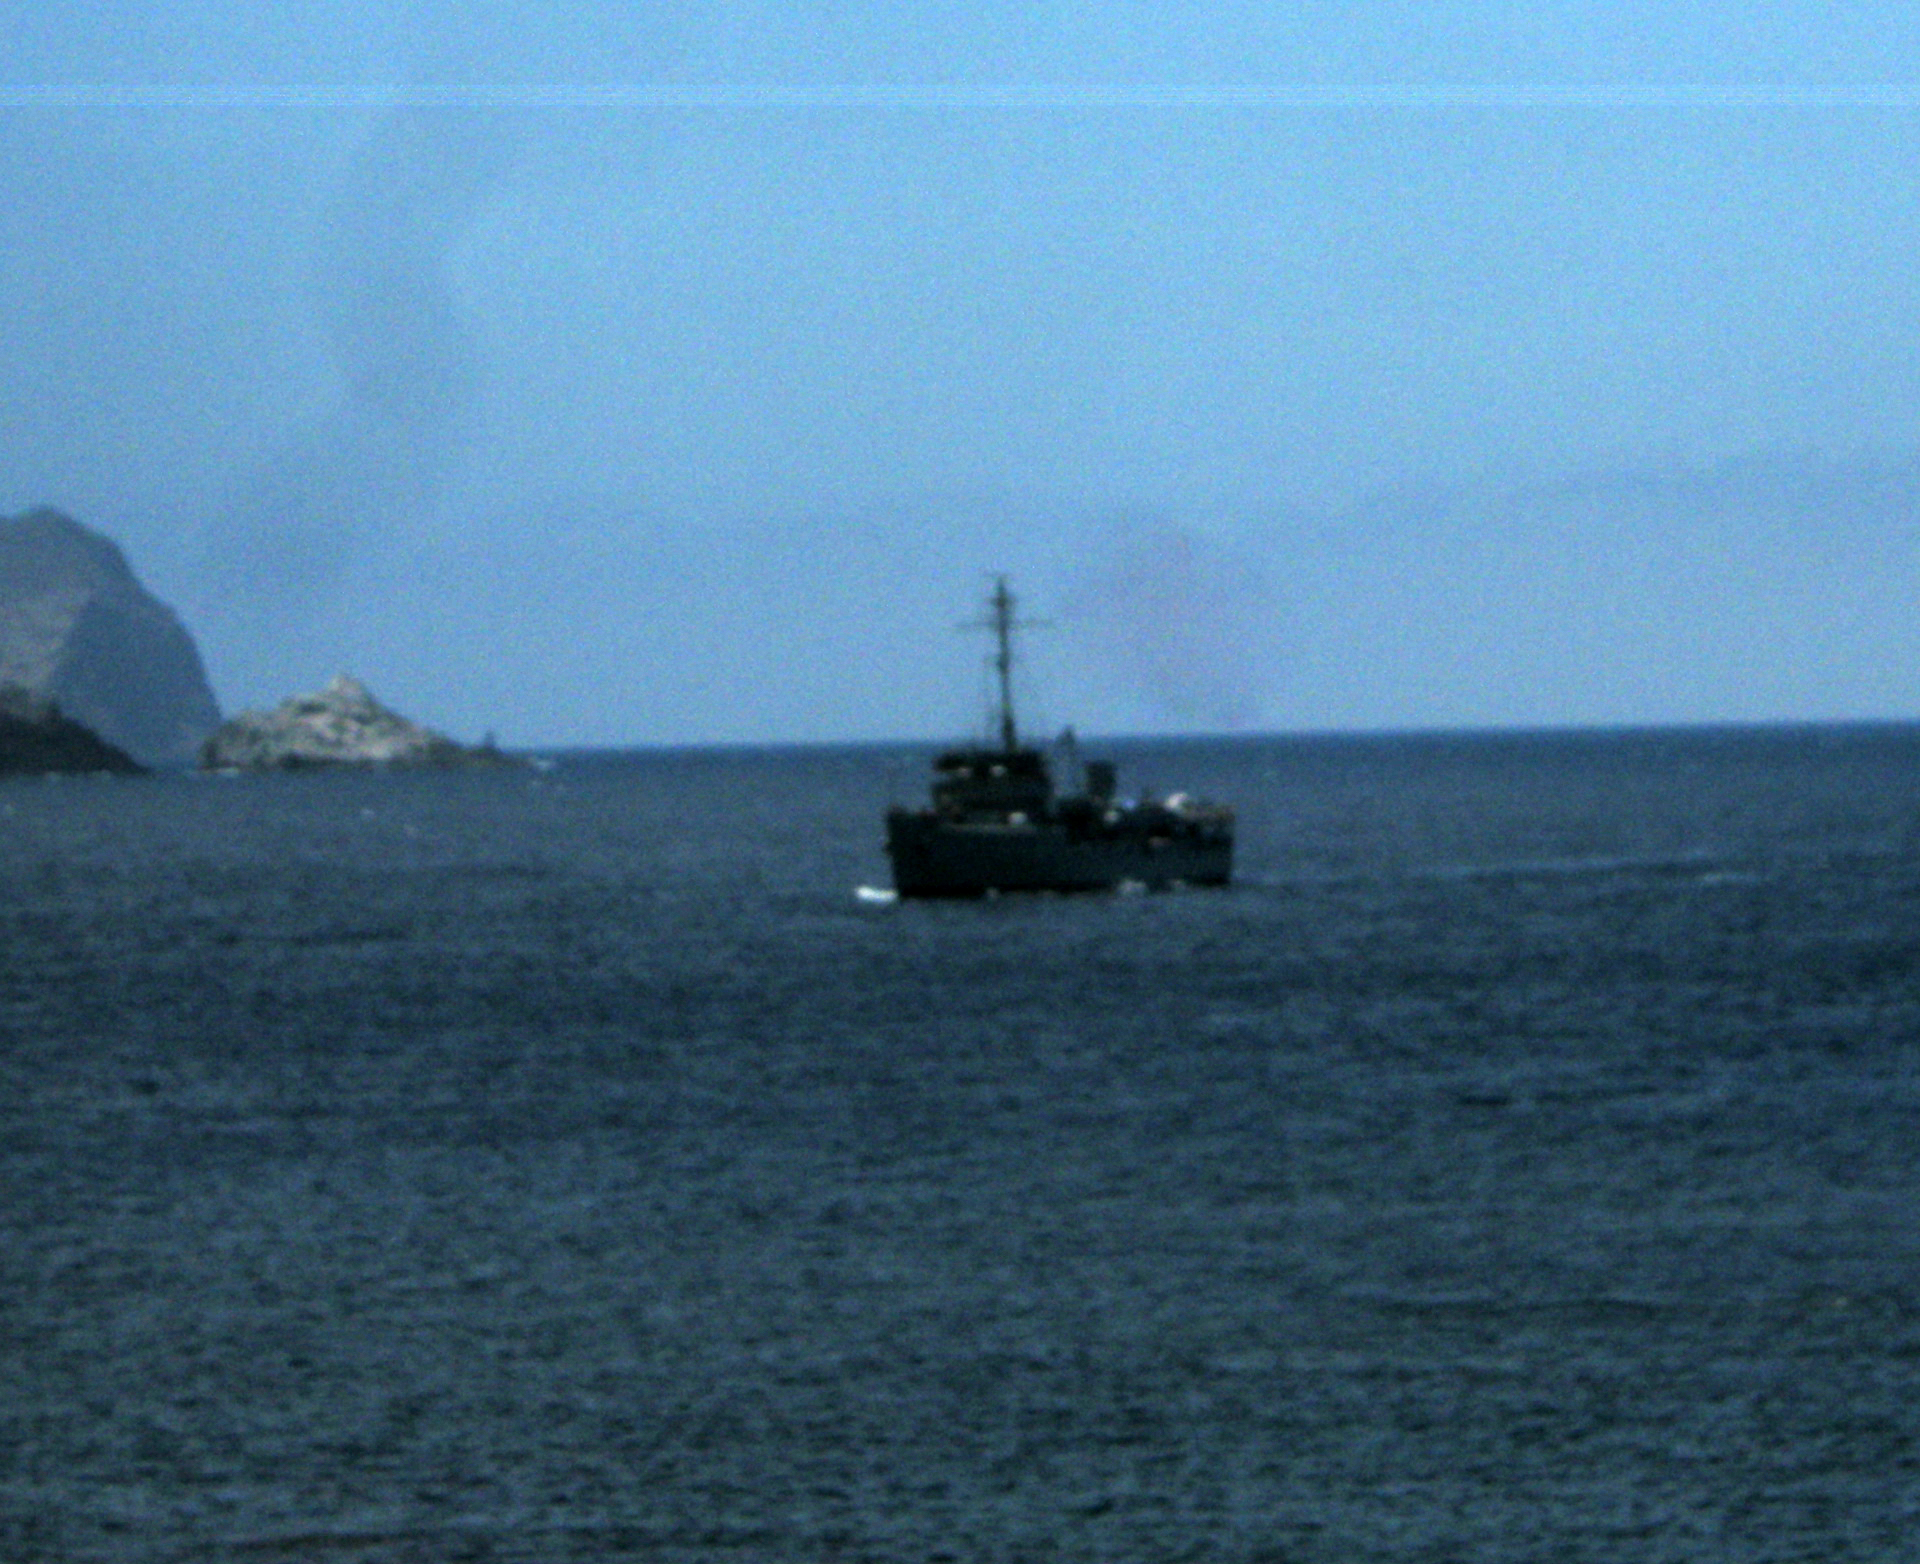
\includegraphics[width=0.95\linewidth]{RFI_testing/figures/mex_navy_arrival.jpg}
\caption{Mexican naval vessel as it arrived at Isla Guadalupe to deliver supplies and pick us up.}
\label{Fig:guadboat}
\end{minipage}%
\begin{minipage}[b]{0.02\textwidth}
\hspace{1cm}
\end{minipage}%
\begin{minipage}[b]{0.51\textwidth}
\centering
\includegraphics[width=0.95\linewidth]{RFI_testing/figures/mex_navy_onboard.jpg}
\caption{View from on board the Mexican naval vessel during the trip back to the Port of Ensenada.}
\label{Fig:guadonboard}
\end{minipage}
\end{figure}

\subsubsection{Logistics and Current Infrastructure}

Access to Isla Guadalupe requires one of two transport methods. First, small planes such as the one shown in Figure \ref{Fig:guadplane} can fly from the city of Ensenada in Baja California to the island, where there is a small landing strip. This flight takes 1-2 hours and can only be made during good weather. On several of our visits to Isla Guadalupe, this was our method of transport. However, each flight costs about \$2000 and can only carry $\sim$600 $kg$ including both people and supplies. 

A much cheaper alternative is transport with the supply ship that the Mexican Navy uses to support its base on Guadalupe. This supply ship, shown in Figures \ref{Fig:guadboat} and \ref{Fig:guadonboard}, deploys once a month from the port of Ensenada; stopping first at Isla Guadalupe, then Isla Cedros, then returning to Ensenada with a total travel time of about three days. Travel via this route requires passengers to $''$camp out$''$ by sleeping on the deck of the ship during transit. In addition, since passengers are hitching a ride with the ship they have no control over changes in ship deployment (eg delays or re-routing) that may change the departure or arrival schedule. This places strictures on any deployments to Isla Guadalupe that must be accounted for in planning the trip. In comparison to the flight costs, passage on the supply ship is only \$50 per person (for food) with minimal weight limits as some of the other passengers have been known to even transport cars via the supply ship. 

While on Guadalupe we had the option of staying with the ecologists, the fishing village or the navy base. Each provided some level of logistical support, but all had limited resources. 

The ecology camp is a small camp with about 5-15 researchers in residence at any given time. Housing, including running water, is available at the site for the researchers and their visitors but there is little to no plumbing, so the bathroom is a dry toilet.  Since power is supplied by solar panels and batteries, it is pretty limited, especially at night. However, during the day there is regular internet access via satellite. Since it is a small camp, food is served communally, with everyone taking turns for cooking and cleaning responsibilities. 

In contrast, the fishing village has a semi-permanent population of about 100 people and can be seen in Figure \ref{Fig:guadplateau}. The fishing village is a cooperative, which means that resources and profits are shared within the community. Houses are assigned to individual families who are currently living on site, as opposed to their main homes on the mainland. Furnishings in the houses are haphazard since all of the furnishings had to be brought in on boats. There is a sewage plant for the village, but no running water (so flushing the toilet means dumping sea water into the bowl). Instead, water is supplied by a desalination plant and each family has barrels of both clean water and sea water at their homes. 

Power in the village is supplied by a large generator that runs throughout the day, except for a few hour siesta in the mid-afternoon and in the middle of the night. Food supplies are purchased by the cooperative and shipped in via the supply boat. Bulk supplies are stored at the community store where each family can $''$purchase$''$ food by signing out the items they need and debiting the cost to their share of the cooperative's profits. When we stayed in the fishing village, we were given use of one of the houses that was currently unoccupied. Meanwhile, we paid one of the fishermen's wives to cook for us.  

Like the ecology camp, the military (naval) base is extremely minimal in scope. There is only a small contingent of personnel ($\sim$10) at any time, so there are only a few buildings with a small generator and everyone takes turns cooking, etc. Water is also limited at the base, since the only natural water source on the island is located at the peak near the ecology camp. 

\begin{figure}[tb]
\begin{center}
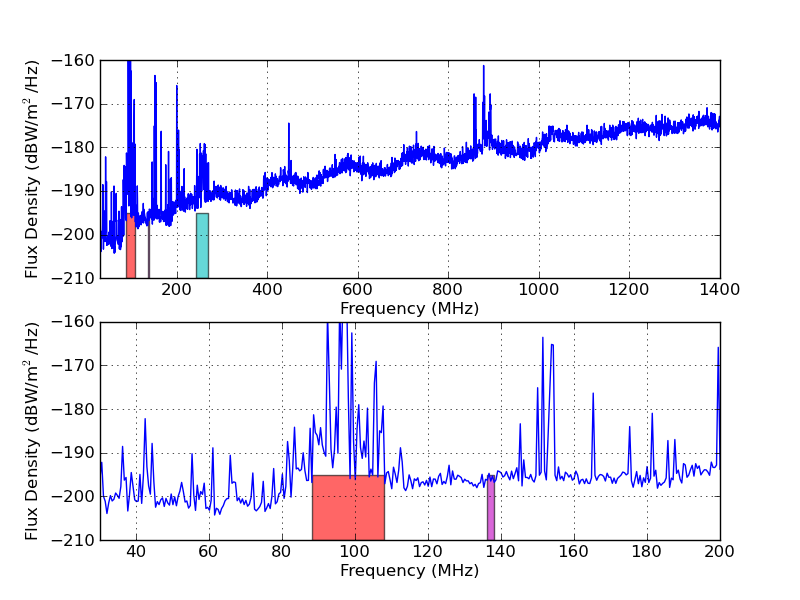
\includegraphics[width=0.9\linewidth]{RFI_testing/figures/GI_3__bands.png}
\caption{RFI measurement from the ecology camp at the summit of Isla Guadalupe collected on November 1st, 2012. At this site, the elevation means that the line of sight is longer and RFI can be seen from further distances than at lower elevations. Despite this fact, the spectrum is mostly free from RFI above $300 MHz$. In the plot, colored boxes again indicate bands of well known RFI sources (Red= FM band, Purple = Orbcomm satellite band, and Cyan = military satellite band).}
\label{Fig:guadsummit}
\end{center}
\end{figure}

\subsubsection{Environmental Impacts}

Located in the Pacific Ocean, in the midst of the California current, Isla Guadalupe is quite temperate for its latitude. The high elevation of its peaks (nearly $1300 \; m$) means that there are two distinct micro-climates (one near sea level and one at high elevations). One reason for this contrast is that the island's peaks sit above the low cloud layer, making the higher altitudes warmer and generally clearer. Additional impacts include flash flooding in the lower areas of the island during the wet season and wind and dust interfering with system at any time. 

Guadalupe's location puts it north of the main Pacific hurricane impact zone, but during the hurricane season storms pass over the island. In addition, the naval supply vessel often has its schedule changed during this season due rough seas from the storms. As an example, we had to change our deployment strategy from boat transit to plane in October 2012 due to Hurricane Paul, which hit the island as a weak tropical depression. This means that the optimal time to visit Isla Guadalupe is during the hurricane off-season (November to June). 


\begin{figure}[htb]
\begin{center}
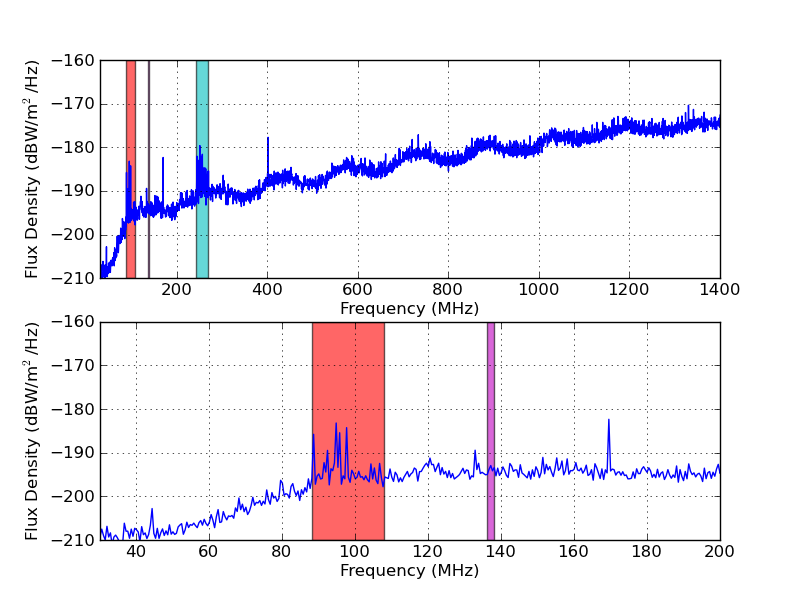
\includegraphics[width=0.9\linewidth]{RFI_testing/figures/GI_2__bands.png}
\caption{RFI measurement from the lava flow near the fishing village at Isla Guadalupe collected on November 1st, 2012. At this site, the lower elevation and the mountain between the lava flow and the mainland act as an RFI shield. This means that even the lowest frequency bands are relatively clear of RFI. In the plot, colored boxes again indicate bands of well known RFI sources (Red= FM band, Purple = Orbcomm satellite band, and Cyan = military satellite band).}
\label{Fig:guadlow}
\end{center}
\end{figure}

\subsubsection{Measurements}

Upon arrival on Guadalupe, several sites were studied for potential deployment. Site 1 was near the ecology camp at the summit of the northern peak of the island, site 2 was near the fishing village on the western side of the island and site 3 was near the military base on the southern tip of the island. The exact positions of these sites are shown in Figure \ref{Fig:guadmap}. I am only showing results from sites 1 and 2 as they have the most dramatic differences in RFI quality. 

Figure \ref{Fig:guadsummit} shows the RFI signals from site 1 at the northern summit. Just as at existing radio quiet sites the spectrum is quite clean at high frequencies. However, as we move to low frequencies there is still some significant RFI, particularly in the FM radio band. Much of this noise is coming from the radio stations in San Diego and Ensenada, including some channels which can actually be heard with a hand-held radio. In this case, the elevation is actually a detriment as the height extends the line of sight for the RFI testing antenna. 

In contrast, Figure \ref{Fig:guadlow} shows the RFI signals from site 2 near the fishing village. Here the combination of low elevation, distance from the mainland and the peaks of Guadalupe act as an excellent shield to minimize the RFI in the FM band to nearly undetectable levels. As seen from the plane in Figure \ref{Fig:guadplateau}, this plateau has significant elevations to the north, south, and east, effectively shielding it from mainland Mexico and Baja California. 

\begin{figure}[htb]
\begin{center}
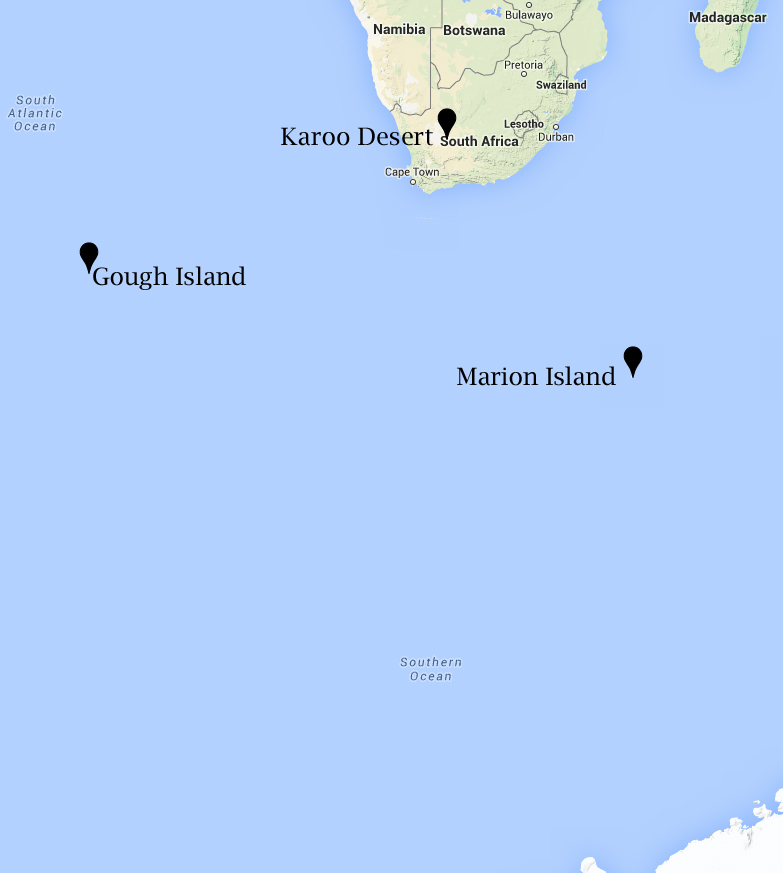
\includegraphics[width=0.7\linewidth]{RFI_testing/figures/site_testing_south_wdesert.jpg}
\caption{Potential future site testing locations in the Southern Hemisphere. Image made using Google Maps.}
\label{Fig:site_map_south}
\end{center}
\end{figure}



\section{Future Sites}

Deployment in June 2013 to Isla Guadalupe with the SCI-HI experiment demonstrated that while the island has very low RFI in general, there is still some residual RFI in the FM band ($88 MHz \leq f \leq 108 MHz$). This RFI makes the band un-usable for the SCI-HI experiment. In order to continue the SCI-HI experiment, several potential sites have been identified.

\begin{enumerate}

\item Isla Socorro and Isla Clari\'{o}n, off the west coast of Mexico, (see Figure \ref{Fig:site_map}) are under investigation as further remote sites in the northern hemisphere.

\item Marion Island, off the coast of South Africa, (see Figure \ref{Fig:site_map_south}) has been identified as an excellent potential site in the southern hemisphere.

\item Additional sites in the southern hemisphere, such as the Antarctic bases and Gough Island, have longer term potential as future sites for testing. 

\end{enumerate}

\subsection{New Sites in Mexico}

Like Isla Guadalupe, Socorro and Clari\'{o}n are small volcanic islands in the Pacific Ocean off the coast of Mexico. Isla Socorro ($18^\circ 47' 4''$ N, $110^\circ 58' 30''$ W) has an area of $\sim$130 $km^2$ and is about 600 $km$ off the western coast of Mexico. Isla Clari\'{o}n ($18^\circ 22'$ N, $114^\circ 44'$ W) has an area of $\sim$20 $km^2$ and is over 700 $km$ from the mainland.

Possessions of Mexico, both islands are ecological reserves with no permanent population. Both islands also have naval installations, although the base on Socorro is significantly larger than the one on Clari\'{o}n. Access to these islands requires permits from the Mexican government, and can be achieved through passage with the Mexican Navy. The Socorro and Clari\'{o}n bases are supported by twice monthly supply boats, and passage can be arranged with the Navy using these boats. 

Weather plays a significant role in limiting visits to Socorro and Clari\'{o}n because most of the Pacific hurricanes impact the islands each year. Therefore, access for research is limited to the off-season (December to May). Site testing on Socorro and Clari\'{o}n is planned for the future.


\subsection{New Sites in South Africa and Antarctica} \label{Sec:SA_site}

Meanwhile, Marion Island ($46^\circ 52' 34''$ S, $37^\circ 51' 32''$ E) is a small volcanic island in the sub-Antarctic Indian Ocean owned by South Africa (see Figure \ref{Fig:site_map_south}). It has an area of $\sim$ 225 $km^2$, with a single peak $\sim$1 $km$ in height. Located $>$2000 $km$ from the South African coast, this island is expected to have excellent isolation from RFI in the FM band. 

Access to the island is provided by the South African National Antarctic Programme (SANAP), which oversees research done on Marion and other islands. Most of the research on the island is focused on the native species and climate. Travel to the island happens once a year, with most of the research occurring over the $\sim$1 month deployment. A small crew remains on the island over the rest of the year ($\sim$11 months). 

Professor Jonathan Sievers at the University of Kwa-Zulu Natal in South Africa was recently awarded a grant through SANAP to investigate and use Marion Island as a site for radio astronomy. As a part of this grant, I will be traveling to Marion Island on the 2016 SANAP trip, which takes place from April to May 2016. During this trip, I will make measurements around the island. These measurements will be used to evaluate the overall RFI environment and identify the best location to place an experiment. I will also deploy the SCI-HI experiment at the location I identify during my evaluation. 

Since this trip is over a year away, we will deploy the SCI-HI instrument to the Karoo desert in South Africa in April 2015. The Karoo desert site is the future location for the Square Kilometer Array \cite{ska} in South Africa, and as such is a protected radio quiet site. The Karoo site is not expected to be as quiet in the FM band as Marion island, but is much more readily accessible.  

